\section{Interview 15 Abridged Transcript with Interaction Designer }

\begin{figure}[h]
\centering
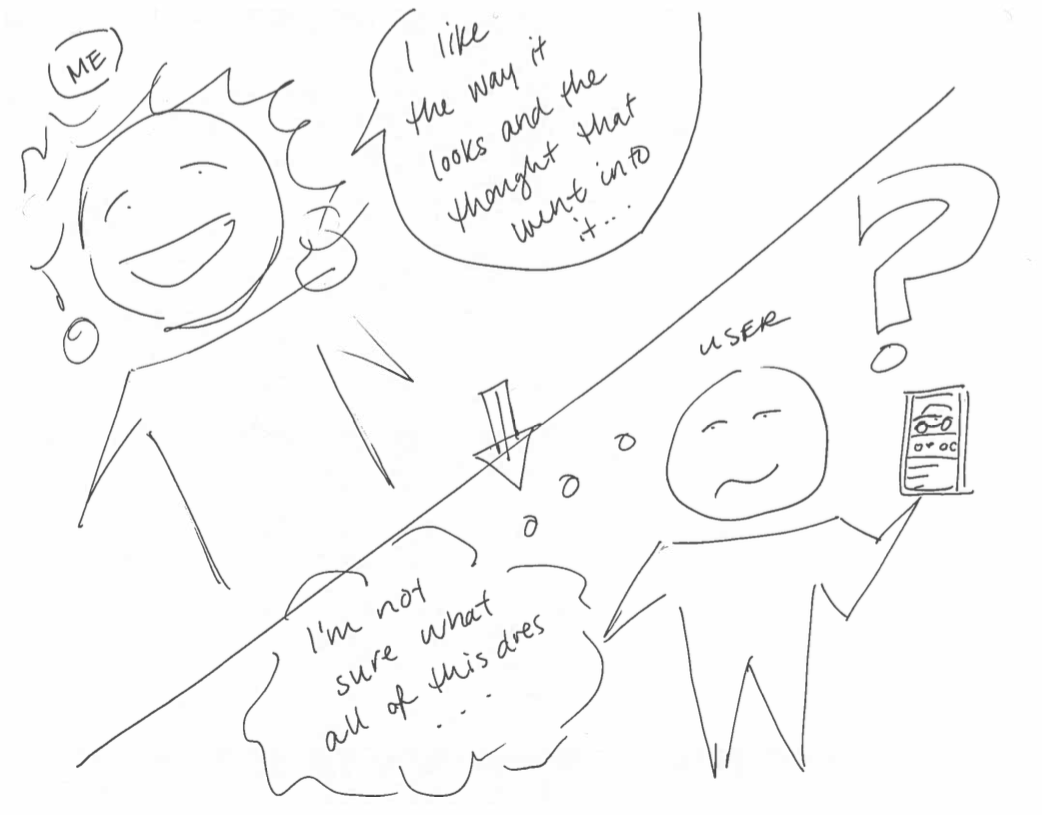
\includegraphics[width=6.5in]{interviews/drawings/2016_01_08.png}
\caption{\quotes{2016-01-08 Interaction Designer's drawing of software development process}}
\label{2016_01_08}
\end{figure}

\textbf{Todd:} My first question for you is very open ended.  00:02

\textbf{Interviewee:} Okay.  00:03

\textbf{Todd:} There is no wrong answer.  I was hoping if you could draw how you feel about the product.  00:09

\textbf{Interviewee:} Okay.  This may get elaborate.  00:27

\textbf{Todd:} Fantastic.  00:29

\textbf{Interviewee:} This is my new pen so.  [Pause] Here we are.  I did sort of a story board-ish type of thing.  02:54

\textbf{Todd:} I love it.  02:55

\textbf{Interviewee:} So, do you want me to explain it?  02:58

\textbf{Todd:} Please.  02:58

\textbf{Interviewee:} Okay.  On one hand superficially, I'm happy because aesthetically, I think it's nice.  I think it's, when you compare it to some of the projects we do, it's been going on for so long and there's such a huge team of smart people.  I feel like we got so much done and it's complex and interesting and there's lot of thought that went into it and it's a really robust app but I'm worried that even though it's pretty and we built a lot of features and the technology is cool, not all of it is necessarily useful for end users and I didn't even give the user name anything because I don't even know that we're designing for the right person all the time with some of our features.  I don't know.  So, I'm worried there were will be more confusion in the marketplace than I would like there to be in a product that I've worked on.  03:57

\textbf{Todd:} Anything else?  04:01

\textbf{Interviewee:} In the drawing or in general?  04:05

\textbf{Todd:} Both.  04:06

\textbf{Interviewee:} Not so much in the drawing.  I guess the big question mark is just that I don't know, I think it's pretty usable but I'm worried there's going to be features for the users or going to be like what is this or why do I care or they'll have question marks around there's something really obvious to me like \ldots I would like you heard a lot of feedback, I want a light telling me if my oil is low and that's just not something we could do because of constraints on the technology I think.  So, I'm worried if people will look at it and say why is there all this stuff that I don't want and there's some stuff that maybe feels really obvious to some users that we haven't provided for one reason or another but overall, I still feel happy.  I think we created a solid product.  04:59

\textbf{Todd:} Good.  When you were describing your \quotes{you} picture, you used the word \quotes{superficially}.  I don't remember the exact word but something like given this superficially I feel happy about it and I was curious if there was like an under feeling of the product.  05:17

\textbf{Interviewee:} Yeah, currently to some degree, this is the under feeling.  The superficial part is a little bit as a designer is a normal person walking around, you feel like people look at it and like it's so beautiful and that might be the beginning and the end of what they think of the app.  They might not use it.  Maybe, it's not for them.  I feel like I could put it in a portfolio or take some of those App Store screens and show it to people and maybe like oh my God, this is the nicest product, you must have done a great job or your team must have worked really hard but if we built something that's really beautiful but doesn't meet the needs of our users, it's kind of I'm still superficial.  I guess part of me is still happy it's beautiful at least or that there's parts of it that are really pretty but at the end of the day as a designer, it's kind of a big fail to build something that's pretty but not the right thing.  It should be a big fail for everybody but especially as the designer, that's what you want to avoid.  06:21